% !TEX root = ../enac_project_fr.tex
\chapter{Modélisation et mise en œuvre du positionnement GNSS}
\label{chap:modelisation}

Ce chapitre présente les modèles nécessaires au calcul de la position d'un
récepteur GNSS. Le but est de commencer dans un premier temps par l'algorithme SPP, puis de d'apporter les améliorations nécessaires pour un algorithme de PPP.
Le chapitre présente les modèles physiques utilisés, ainsi que leur mise en œuvre dans Orekit.
Les détails de la résolution mathématique des équations de positionnement sont donnés en annexe~\ref{ann:estimation}.

\section{Positionnement par SPP}

Cette section présente la théorie du positionnement par \emph{Single Point Positioning} qui sera retenue puis implémentée dans ce travail.

\subsection{Principe théorique}

La pseudo-distance est obtenue en estimant le décalage temporel entre le code
reçu et une réplique du même code générée par le récepteur. Cette pseudo distance doit être corrigée
pour tenir compte des différents biais et retard qui l'affectent, et qui faussent la valeur réelle de la distance.
Ces corrections peuvent être liées à des effets atmosphériques, à la rotation de la Terre, ou à des biais d'horloge, et toutes n'ont pas
le même ordre de grandeur. Dans une résolution par SPP, on tient compte des effets les plus significatifs, de sorte à avoir une estimation 
dont la précision est de l'ordre du mètre. Les effets les plus faibles sont négligés et seront pris en compte dans les parties ultérieures.
Pour le récepteur
$r$, le satellite $s$ et la fréquence $i$, elle est modélisée en mètres par

\begin{align}
P_{r,i}^s &=
\rho_r^s+c(\delta t_r-\delta t^s)+T_r^s+I_{r,i}^s
+\delta_{\mathrm{Sagnac},r}^s
+\varepsilon_{P,r,i}^s.
\label{new:code}
\end{align}
avec :
\begin{itemize}
    \item $P_{r,i}^s$ la pseudo-distance mesurée 
    \item $r$, $s$ et $i$ les indices du récepteur, du satellite et de la
    fréquence 
    \item $\rho_r^s=\|\mathbf r^s-\mathbf r_r\|$ la distance géométrique 
    \item $\mathbf r^s$ et $\mathbf r_r$ les positions du satellite et du
    récepteur dans un même repère 
    \item $\delta t_r$ et $\delta t^s$ les biais d'horloge du récepteur et du
    satellite 
    \item $T_r^s$ le retard troposphérique 
    \item $I_{r,i}^s$ le retard ionosphérique 
    \item $\delta_{\mathrm{Sagnac},r}^s$ la correction de Sagnac 
    \item $\varepsilon_{P,r,i}^s$ l'erreur de la mesure de code.
\end{itemize}


Les coordonnées sont exprimées dans un repère terrestre.

Les détails de ces termes de correction seront étudiés dans la
section~\ref{new:corrections}. L'équation~\eqref{new:code} peut être réécrite en
distinguant les termes que l'on peut évaluer des paramètres inconnus :

\begin{align}
\underbrace{
P_{r,i}^s
+c\delta t^s
-T_r^s
-I_{r,i}^s
-\delta_{\mathrm{Sagnac},r}^s
}_{\text{Pseudo-distance corrigée }\overline P_r^s}
&=
\rho_r^s+c\delta t_r+\varepsilon_{P,r,i}^s.
\label{eq:termes_eval}
\end{align}

\subsection{Corrections utilisées en SPP}
\label{new:corrections}

L'un des principaux termes affectant les observations GNSS provient des imperfections des horloges embarquées à bord des satellites et de celle du récepteur. 
Comme le signal électromagnétique émis par les satellites se propage dans le vide à la vitesse de la
lumière c, une erreur d'une microseconde correspond à une erreur de distance d'environ 300 m.   

\begin{align}
1\,\text{µs} &\leftrightarrow 300\,\text{m}
\end{align}
\subsubsection{Horloge satellite}

Les satellites GNSS sont équipés d'horloges atomiques très stables, mais celles-ci présentent malgré tout un biais et une dérive qui évoluent au cours du temps. Les paramètres permettant de modéliser cette évolution sont transmis dans le message de navigation émis par les satellites.

Pour chaque satellite, le biais d'horloge est modélisé par un polynôme du second ordre~\cite{isgps200n} :

\begin{align}
\delta t_{\mathrm{poly}}^s(t)
=
a_{f0}^s
+
a_{f1}^s(t-t_{oc}^s)
+
a_{f2}^s(t-t_{oc}^s)^2,
\end{align}

où

\begin{itemize}
    \item $t$ est l'instant considéré ;
    \item $t_{oc}^s$ est l'époque de référence des paramètres d'horloge du
    satellite $s$ ;
    \item $a_{f0}^s$, $a_{f1}^s$ et $a_{f2}^s$ sont respectivement le biais,
    la dérive et la dérive seconde de l'horloge. Ces coefficients sont fournis
    dans le fichier RINEX Navigation.
\end{itemize}

Il faut également tenir compte d'une correction relativiste liée à l'excentricité de l'orbite du satellite~\cite{ashby2003}, donnée par

\begin{align}
\Delta t_{\mathrm{rel}}^s
=
-\frac{2}{c^2}\,
\mathbf r^s \cdot \mathbf v^s
=
-2\frac{\sqrt{\mu a}\,e}{c^2}\,\sin E,
\end{align}

avec :
\begin{itemize}
    \item $\mathbf r^s$ et $\mathbf v^s$ respectivement la position et la
    vitesse du satellite $s$ ;
    \item $\mu$  la constante gravitationnelle standard de la Terre ;
    \item $a$ le demi-grand axe de l'orbite ;
    \item $e$ son excentricité ;
    \item $E$ l'anomalie excentrique.
\end{itemize}

Le biais d'horloge satellite total est obtenu en combinant le polynôme
diffusé et la correction relativiste :

\begin{align}
\delta t^s(t) = \delta t_{\mathrm{poly}}^s(t)
+ \Delta t_{\mathrm{rel}}^s.
\label{eq:broadcast_satellite_clock}
\end{align}

avec :

\begin{itemize}
    \item $\delta t^s$ le biais d'horloge du satellite $s$ par rapport au
    temps du système ;
    \item $\delta t_{\mathrm{poly}}^s$ le terme polynomial diffusé ;
    \item $\Delta t_{\mathrm{rel}}^s$ la correction relativiste liée à
    l'excentricité orbitale.
\end{itemize}

À cela s'ajoute, dans certains cas, un terme de \textit{Total Group Delay}
(TGD), diffusé dans le message de navigation~\cite{isgps200n}. Il représente un biais de groupe propre au signal de code. Pour une
convention de type GPS, le biais d'horloge apparent associé à la fréquence
$f_i$ s'écrit

\begin{align}
\delta t_i^s
&=
\delta t^s-\gamma_i\,\delta t_{\mathrm{TGD}}^s,
&
\gamma_i
&=
\frac{f_1^2}{f_i^2}.
\label{eq:tgd_signal_clock}
\end{align}

avec :

\begin{itemize}
    \item $\delta t_i^s$ le biais apparent utilisé pour l'observation de code
    sur la fréquence $i$ ;
    \item $\delta t_{\mathrm{TGD}}^s$ le TGD diffusé par le satellite $s$ ;
    \item $\gamma_i$ le facteur de changement de fréquence.
\end{itemize}

Le nom du paramètre, sa fréquence de référence et son signe dépendent de la
constellation : Galileo diffuse notamment des BGD~\cite{galileoOsSisIcd21}. Le TGD ou le BGD doit donc
être appliqué selon le signal de code utilisé. Il ne s'applique pas comme un
terme d'horloge commun à la phase. Avec des produits précis CLK et BIA, les
conventions des horloges et des biais observables remplacent ce traitement
diffusé.

\subsubsection{Horloge récepteur}

Le biais d'horloge du récepteur, quant à lui, est inconnu et ne peut être corrigé a priori. Il constitue donc un paramètre supplémentaire dans le vecteur d'état, estimé conjointement avec les coordonnées du récepteur au cours de la résolution.

\subsubsection{Effet Sagnac}\label{sagnac}

Cet effet découle de la rotation terrestre pendant la propagation du signal et
de la transformation entre repères inertiel et terrestre~\cite{ashby2003}.

Pendant le temps nécessaire à la propagation du signal GNSS, de l'ordre de 70 ms, la Terre poursuit sa rotation autour de son axe. Le satellite émet donc son signal dans une position exprimée dans un repère terrestre qui a légèrement tourné lorsque le signal est reçu. 

La correction de Sagnac s'écrit

\begin{align}
\delta_{\mathrm{Sagnac},r}^s
=
\frac{1}{c} (\boldsymbol\omega_E \times \mathbf r^s)\cdot\mathbf r_r
=
\frac{\omega_E}{c}
\left(
x^s y_r
-
y^s x_r
\right),
\end{align}

où

\begin{itemize}
    \item $\mathbf r^s$ et $\mathbf r_r$ sont respectivement les vecteurs position du satellite et du récepteur dans le repère terrestre ;
    \item $\boldsymbol\omega_E$ est le vecteur de rotation de la Terre ;
    \item $(x^s,y^s)$ sont les coordonnées du satellite dans le repère terrestre ;
    \item $(x_r,y_r)$ sont les coordonnées du récepteur ;
    \item $c$ est la vitesse de la lumière.
\end{itemize}

\subsubsection{Modélisation de la troposphère}

Les signaux GNSS traversent la troposphère avant d'atteindre le récepteur.
Cette couche de l'atmosphère, composée principalement d'air sec et de vapeur
d'eau, possède un indice de réfraction légèrement supérieur à celui du vide.
La vitesse de propagation des ondes électromagnétiques y est donc légèrement
réduite, ce qui se traduit par un retard de propagation qui affecte directement
les mesures de pseudo-distance et de phase.

Le retard troposphérique dépend principalement de la pression, de la
température et de la teneur en vapeur d'eau de l'atmosphère. Il est
classiquement décomposé selon le modèle de Saastamoinen~\cite{saastamoinen1972} en une composante hydrostatique (\textit{dry}),
relativement stable, et une composante humide (\textit{wet}), plus variable.
Le retard troposphérique au zénith, appelé \textit{Zenith Total Delay} (ZTD),
s'écrit ainsi
\begin{align}
ZTD = ZHD + ZWD,
\label{eq:ztd_decomposition}
\end{align}
où $ZHD$ (\textit{Zenith Hydrostatic Delay}) désigne le retard hydrostatique
au zénith et $ZWD$ (\textit{Zenith Wet Delay}) le retard humide au zénith.

Lorsque l'atmosphère est supposée symétrique autour du récepteur, le retard ne
dépend que de l'élévation du satellite. Le modèle de base s'écrit

\begin{align}
T_{r,0}^s(E_r^s)
=
M_{\mathrm{dry}}(E_r^s)ZHD
+
M_{\mathrm{wet}}(E_r^s)ZWD.
\label{eq:tropo_no_grad}
\end{align}

avec :

\begin{itemize}
    \item $T_{r,0}^s$ le retard troposphérique 
    \item $E_r^s$ l'angle d'élévation du satellite $s$ vu par le récepteur
    $r$ 
    \item $M_{\mathrm{dry}}$ et $M_{\mathrm{wet}}$ les fonctions de projection
    des composantes hydrostatique et humide 
    \item $ZHD$ et $ZWD$ les retards hydrostatique et humide au zénith
\end{itemize}

Les fonctions de projection permettent de relier les retards mesurés selon
la direction du satellite aux retards correspondants au zénith. Pour les traitements utilisant la projection de Niell, les fonctions de projection du modèle \textit{Niell Mapping Function}~\cite{niell1996}
(NMF) sont utilisées. Leur formulation détaillée est présentée en
annexe~\ref{annexe:nmf}.

La composante hydrostatique représente la majeure partie du retard
troposphérique et varie relativement lentement. Elle peut être calculée à
partir de la pression atmosphérique au niveau du récepteur. Une expression
couramment utilisée est
\begin{align}
ZHD
=
\frac{0.0022768\,P}
{1-0.00266\cos(2\varphi)-2.8\times10^{-7}h},
\label{eq:zhd}
\end{align}
où $P$ est la pression atmosphérique exprimée en hPa, $\varphi$ la latitude
géographique du récepteur et $h$ son altitude.

Dans le traitement SPP retenu, les composantes hydrostatique et humide sont
calculées de manière déterministe en utilisant l'équation \ref{eq:tropo_no_grad}. 

\subsubsection{Correction ionosphérique}

Avant d'atteindre le récepteur, les signaux GNSS traversent également
l'ionosphère, région de la haute atmosphère contenant une importante
concentration d'électrons libres. La présence de ces électrons modifie
l'indice de réfraction du milieu et affecte ainsi la propagation des ondes
électromagnétiques. Contrairement au retard troposphérique, cet effet est
dispersif : son amplitude dépend de la fréquence du signal et est, au
premier ordre, inversement proportionnelle au carré de celle-ci~\cite{hauschild2017observations}.

Pour une fréquence $f_i$, le retard ionosphérique entre le satellite $s$ et le
récepteur $r$ peut
ainsi être exprimé sous la forme

\begin{align}
I_{r,i}^s
\propto
\frac{1}{f_i^2}.
\end{align}

Deux approches sont considérées dans cette étude. Pour le positionnement
monofréquence, le retard ionosphérique est modélisé à l'aide du modèle de
Klobuchar. Pour le positionnement bi-fréquence, l'effet ionosphérique du
premier ordre est supprimé par l'utilisation d'une combinaison
\textit{iono-free}.

\subsubsection{Modèle de Klobuchar}

Le modèle de Klobuchar est un modèle empirique de l'ionosphère conçu
initialement pour fournir une correction de propagation à faible coût
calculatoire aux utilisateurs GPS monofréquence. Il constitue le modèle
ionosphérique diffusé directement dans le message de navigation GPS~\cite{klobuchar1987} et
permet d'obtenir une estimation du retard ionosphérique sur la fréquence
L1.

Pour une observation donnée, le modèle utilise comme entrées la latitude et
la longitude approximatives du récepteur, l'élévation et l'azimut du
satellite, le temps GPS ainsi que les huit coefficients $\alpha_0,\ldots,
\alpha_3$ et $\beta_0,\ldots,\beta_3$ transmis dans le message de navigation.
Ces coefficients permettent de caractériser l'amplitude et la période de la
variation temporelle du retard ionosphérique. 

Le principe du modèle consiste à représenter l'ionosphère par une couche
mince située à une altitude conventionnelle, puis à déterminer le point
d'intersection du signal avec cette couche, appelé \textit{Ionospheric
Pierce Point} (IPP). Le retard vertical estimé à cet endroit est ensuite
projeté sur la direction du satellite afin d'obtenir le retard
ionosphérique selon la ligne de visée.

Les différentes étapes de calcul ainsi que les équations détaillées du
modèle sont présentées en annexe~\ref{Klobuchar}.

\subsubsection{Combinaison iono-free}

La combinaison iono-free consiste (IF) à effectuer une combinaison linéaire des mesures de code et de phase, de
sorte à éliminer le retard
ionosphérique au premier ordre. 

Pour les mesures de code $P_{r,1}^s$ et $P_{r,2}^s$, la combinaison
\textit{iono-free} est définie par

\begin{align}
P_{r,\mathrm{IF}}^s
=
\frac{
f_1^2P_{r,1}^s-f_2^2P_{r,2}^s
}{
f_1^2-f_2^2
}.
\label{eq:code_iono_free}
\end{align}

La même combinaison sera utilisée en PPP pour la phase,
notée $L_{r,i}^s$ en mètres :

\begin{align}
L_{r,\mathrm{IF}}^s
=
\frac{
f_1^2L_{r,1}^s-f_2^2L_{r,2}^s
}{
f_1^2-f_2^2
}.
\label{eq:phase_iono_free}
\end{align}

Considérons par exemple le modèle simplifié

\begin{align}
P_{r,i}^s
&=
\mathcal G_r^s
+
I_{r,i}^s
+
\varepsilon_{P,r,i}^s
\end{align}

avec $\mathcal G_r^s$ l'ensemble des termes indépendants de la fréquence :

\begin{align}
\mathcal G_r^s
&=
\rho_r^s
+c\left(\delta t_r-\delta t^s\right)
+T_r^s
+\delta_{\mathrm{Sagnac},r}^s
,
\label{eq:common_nondispersive_term}
\end{align}

et le retard ionosphérique du premier ordre

\begin{align}
I_{r,i}^s
=
\frac{K_r^s}{f_i^2},
\qquad
K_r^s=40{,}3\,\mathrm{STEC}_r^s,
\end{align}

avec :

\begin{itemize}
    \item $B_{r,i}^s=\lambda_iN_{r,i}^s$ l'ambiguïté métrique de phase 
    \item $\varepsilon_{P,r,i}^s$ et $\varepsilon_{L,r,i}^s$ les erreurs
    résiduelles de code et de phase 
    \item $\mathrm{STEC}_r^s$ le contenu électronique total intégré le long
    du trajet satellite--récepteur, exprimé en électrons par mètre carré 
    \item $K_r^s=40{,}3\,\mathrm{STEC}_r^s$ le coefficient ionosphérique du
    premier ordre, indépendant de la fréquence $f_i$. Le facteur $40{,}3$
    est exprimé en $\mathrm{m^3\,s^{-2}}$ lorsque $I_{r,i}^s$ est en mètres,
    $\mathrm{STEC}_r^s$ en électrons par mètre carré et $f_i$ en Hz.
\end{itemize}

En substituant cette expression dans l'équation~\eqref{eq:code_iono_free},
le terme ionosphérique devient

\begin{align}
\frac{
f_1^2I_{r,1}^s-f_2^2I_{r,2}^s
}{
f_1^2-f_2^2
}
&=
\frac{
f_1^2\frac{K_r^s}{f_1^2}
-
f_2^2\frac{K_r^s}{f_2^2}
}{
f_1^2-f_2^2
}
\\
&=
0.
\end{align}

Le même raisonnement s'applique à la combinaison des mesures de phase.

Les effets ionosphériques d'ordre
supérieur ne sont pas parfaitement éliminés mais sont négligeables devant le bruit pour du SPP et du PPP.



Les coefficients de la combinaison sont notés
\begin{align}
\alpha=\frac{f_1^2}{f_1^2-f_2^2},\qquad
\beta=-\frac{f_2^2}{f_1^2-f_2^2}.
\label{new:if}
\end{align}
avec :
\begin{itemize}
\item $\alpha$ le coefficient de l'observation sur la première fréquence ;
\item $\beta$ le coefficient de l'observation sur la seconde fréquence.
\end{itemize}

En contrepartie, le bruit de mesure est amplifié :

\begin{align}
\sigma_{P,\mathrm{IF}}^2&=\alpha^2\sigma_{P,1}^2+\beta^2\sigma_{P,2}^2.
\label{new:if_variance}
\end{align}
avec :
\begin{itemize}
\item $\sigma_{P,1}^2$ et $\sigma_{P,2}^2$ les variances des mesures de code ;
\item $\sigma_{P,\mathrm{IF}}^2$ la variance de leur combinaison.
\end{itemize}

\subsection{Estimation de la position SPP}

L'étape de résolution consiste à construire un système d'équations linéaires à partir des mesures de code 
pour estimer la position et le biais d'horloge du récepteur.
Pour cela, 
le SPP utilise les moindres carrés pondérés itératifs ~\cite{verhagen2017least} :
\begin{align}
\widehat{\mathbf x}
&=\mathop{\mathrm{arg\,min}}_{\mathbf x}
[\mathbf y-\mathbf h(\mathbf x)]^{\mathsf T}\mathbf R^{-1}
[\mathbf y-\mathbf h(\mathbf x)],\\
\mathbf x&=[\,x\quad y\quad z\quad c\delta t_r\,]^{\mathsf T}.
\label{new:wls}
\end{align}
avec :
\begin{itemize}
\item $\mathbf y$ le vecteur des observations 
\item $\mathbf h(\mathbf x)$ les observations calculées 
\item $\mathbf R$ la covariance des erreurs d'observation 
\item $\widehat{\mathbf x}$ l'état estimé
\end{itemize}

Une observation de variance élevée reçoit moins de poids. L'état est ajusté
par itérations, indépendamment à chaque époque. La linéarisation, les
équations de résolution et le critère d'arrêt sont détaillés en
annexe~\ref{ann:estimation}.

\subsubsection{Traitement multi-constellation}

L'utilisation de plusieurs constellations augmente le nombre de satellites
disponibles et donc le nombre d'observations. Elle peut améliorer la
géométrie, c'est à dire avoir une répartition plus uniforme des satellites dans le ciel, ce qui améliore la précision de la solution. 
Comme les satellties de deux constellations différentes ont des horloges référencées à leur propre temps, 
il est nécessaire de faire des ajustements détaillés ci-dessous.

Pour Galileo et GPS, le message de navigation fournit le décalage déterministe
entre les deux échelles de temps, appelé GGTO (\textit{Galileo-to-GPS Time
Offset})~\cite{galileoOsSisIcd21}. Il est modélisé par

\begin{align}
\Delta t_{\mathrm{GGTO}}(t)
=
a_0+a_1\left(t-t_{\mathrm{ref}}\right).
\label{eq:ggto}
\end{align}

avec :

\begin{itemize}
    \item $\Delta t_{\mathrm{GGTO}}(t)$ le décalage Galileo--GPS à l'époque
    $t$, en secondes ;
    \item $a_0$ le décalage à l'époque de référence, en secondes ;
    \item $a_1$ sa dérive temporelle, en secondes par seconde ;
    \item $t_{\mathrm{ref}}$ l'époque de référence du message.
\end{itemize}

Ces trois paramètres sont extraits du fichier RINEX Navigation. 
Avec la convention retenue, une observation Galileo
exprimée en mètres est ramenée au temps GPS selon

\begin{align}
O_{r,i}^{s,\mathrm{GPS}}(t)
=
O_{r,i}^{s,\mathrm{GAL}}(t)
-c\,\Delta t_{\mathrm{GGTO}}(t).
\label{eq:ggto_observation_correction}
\end{align}

avec :

\begin{itemize}
    \item $O_{r,i}^{s,\mathrm{GAL}}$ l'observation Galileo avant correction,
    qu'il s'agisse du code ou de la phase exprimée en mètres 
    \item $O_{r,i}^{s,\mathrm{GPS}}$ la même observation ramenée à l'échelle
    de temps GPS 
    \item $c$ la vitesse de la lumière.
\end{itemize}

Par ailleurs, il est aussi nécessaire de prendre en compte les biais inter-systèmes.
Les biais inter-systèmes (ISB, \textit{Inter-System Bias}) représentent des délais hardware propres à chaque constellation, et qui sont des inconnues
supplémentaires à estimer.

Une constellation est choisie comme référence, ici GPS. Pour toute autre
constellation $q$, on introduit un ISB exprimé en mètres :

\begin{align}
c\delta t_{r,q}
&=
c\delta t_r+\mathrm{ISB}_{r}^{q},
&
\mathrm{ISB}_{r}^{\mathrm{GPS}}
&=0,
\\
c\left(\delta t_{r,q}-\delta t^{s,q}\right)
&=
c\left(\delta t_r-\delta t^{s,q}\right)
+\mathrm{ISB}_{r}^{q}.
\label{eq:isb_definition}
\end{align}

avec :

\begin{itemize}
    \item $c\delta t_{r,q}$ le biais d'horloge récepteur effectif pour les
    observations de la constellation $q$ 
    \item $c\delta t_r$ le biais d'horloge commun, défini par rapport au temps
    GPS 
    \item $\delta t^{s,q}$ le biais de l'horloge du satellite $s$, exprimé par
    rapport à l'échelle de temps de la constellation $q$ 
    \item $\mathrm{ISB}_{r}^{q}$ le décalage de la constellation $q$ par
    rapport à la référence. Il regroupe l'écart résiduel entre les échelles de
    temps et les retards différentiels du récepteur.
\end{itemize}

Le terme $\mathrm{ISB}_{r}^{q}$ est ajouté au modèle calculé des observations
de la constellation concernée. Il est inconnu et doit être estimé avec la
position et l'horloge. Pour un traitement GPS--Galileo, le vecteur d'état
minimal pour le SPP devient

\begin{align}
\mathbf x
=
\begin{bmatrix}
x & y & z &
c\delta t_r &
\mathrm{ISB}_{r}^{\mathrm{GAL}}
\end{bmatrix}^{\mathsf T}.
\label{eq:multiconstellation_state}
\end{align}

\section{Positionnement par PPP}

La précision du SPP reste limitée par le bruit du code, les données
diffusées et les erreurs résiduelles des corrections. Le PPP exploite la
phase de porteuse et des données plus précis sur les positions des satellites pour réduire ces limitations.
Le traitement par PPP permet une précision de l'ordre de quelques centimètres.

\subsection{Mesure de phase et ambiguïté}
\label{new:phase_section}

Le code est transporté par une onde sinusoïdale appelée \emph{porteuse}. Le
récepteur compare la phase de l'onde reçue à celle d'une réplique générée par
son oscillateur local. Une fraction de cycle peut ainsi être mesurée avec une grande
finesse ; convertie en distance, cette observation est beaucoup moins bruitée
que la pseudo-distance.

Une mesure de phase seule ne fournit toutefois pas immédiatement la distance
totale. Au moment où le suivi d'un satellite commence, le récepteur mesure la
fraction de cycle courante, mais ignore combien de cycles entiers séparent le
satellite du récepteur. Ce nombre inconnu est l'\emph{ambiguïté entière}. Après acquisition, le récepteur suit les variations de phase et compte les
cycles successifs tant que le suivi reste continu. Ce comptage ne détermine
pas l'ambiguïté initiale. Si $\varphi_{r,i}^s$ désigne la phase accumulée
mesurée, en radians, sa conversion en mètres s'écrit

\begin{align}
L_{r,i}^s
&=
\lambda_i\frac{\varphi_{r,i}^s}{2\pi}.
\label{eq:carrier_phase_definition}
\end{align}

avec :

\begin{itemize}
    \item $L_{r,i}^s$ la mesure de phase convertie en mètres 
    \item $\lambda_i=c/f_i$ la longueur d'onde de la fréquence $f_i$
    \item $\varphi_{r,i}^s$ la phase accumulée mesurée, en radians,
    incluant les cycles comptés depuis l'acquisition.
\end{itemize}

En reprenant les corrections déjà présentées,
le modèle de phase s'écrit~\cite[p.~591]{capderou2012}

\begin{align}
L_{r,i}^s
&=
\rho_r^s
+c\left(\delta t_r-\delta t^s\right)
+T_r^s
-I_{r,i}^s
+\lambda_i N_{r,i}^s
+\delta_{\mathrm{Sagnac},r}^s
+\varepsilon_{L,r,i}^s,
\label{new:phase}
\end{align}

avec :

\begin{itemize}
    \item $B_{r,i}^s=\lambda_i N_{r,i}^s$ l'ambiguïté de phase exprimée
    en mètres, où $N_{r,i}^s$ est l'ambiguïté entière en cycles 
    \item $\delta_{\mathrm{Sagnac},r}^s$ la correction de Sagnac 
    \item les autres termes géométriques, atmosphériques et d'horloge
    définis dans l'équation~\eqref{new:code} ;
    \item $\varepsilon_{L,r,i}^s$ l'erreur résiduelle de phase
\end{itemize}

Le terme ionosphérique apparaît avec un signe opposé à celui du code. En effet le plasma
ionosphérique produit un retard de groupe sur la modulation de code, mais une
avance de phase sur la porteuse. 

Les corrections supplémentaires de Shapiro, d'antenne et de wind-up seront
ajoutées dans la présentation du modèle PPP complet. À ce stade, comme pour
le code, les termes supposés évalués sont placés dans le membre de gauche :

\begin{align}
\underbrace{
L_{r,i}^s
+c\delta t^s
-T_r^s
+I_{r,i}^s
-\delta_{\mathrm{Sagnac},r}^s
}_{\text{Phase corrigée }\overline L_{r,i}^s}
&=
\rho_r^s+c\delta t_r+\lambda_i N_{r,i}^s+\varepsilon_{L,r,i}^s.
\label{eq:phase_corrigee}
\end{align}

avec :

\begin{itemize}
    \item $\overline L_{r,i}^s$ la phase corrigée, en mètres ;
    \item $\lambda_i N_{r,i}^s$ une inconnue constante tant que le suivi de la porteuse
    reste continu ;
    \item les autres termes sont définis précédemment.
\end{itemize}

Dans une solution à ambiguïtés flottantes, $N_{r,i}^s$ est d'abord estimée
comme un paramètre réel. Déterminer ensuite le nombre entier de cycles
compatible avec cette estimation constitue l'étape de résolution entière des
ambiguïtés~\cite{teunissen2017ambiguity}.


Cette écriture de la phase corrigée suppose le retard troposphérique connu.
Lorsqu'il est estimé en PPP, sa partie inconnue reste dans le modèle calculé.
De même, l'identification $B_{r,i}^s=\lambda_iN_{r,i}^s$ suppose des biais
instrumentaux traités séparément ; une ambiguïté flottante peut absorber
les biais résiduels constants.

Contrairement aux pseudo-distances, les mesures de phase d'une seule époque
ne suffisent pas à déterminer la position lorsque chaque satellite apporte
une ambiguïté inconnue. L'utilisation conjointe du code et de la phase permet
d'exploiter la précision de la porteuse tout en estimant les ambiguïtés.
Le code conserve notamment un rôle essentiel lors de l'initialisation pour
séparer la distance, le biais d'horloge et les ambiguïtés. La fixation entière
n'est pas nécessaire pour obtenir une solution PPP flottante.

\subsubsection{Orbites, horloges et biais précis}

Le PPP remplace les éphémérides et horloges diffusées par des produits précis
issus du traitement d'un réseau de stations. Les fichiers SP3 fournissent les
positions des satellites et les fichiers CLK leurs corrections d'horloge.
Ces données sont interpolées pour obtenir les valeurs à l'instant d'émission.

Les biais de signal doivent être cohérents avec les conventions de ces
horloges. Les produits BIA peuvent fournir des biais différentiels (DCB ou DSB)
ou des biais propres à une observable (OSB). Ils permettent de relier les
observations aux références des produits précis ; le TGD diffusé n'est donc
pas ajouté systématiquement. Il faut éviter de corriger deux fois un effet
déjà absorbé dans l'horloge ou dans les paramètres estimés.


\subsection{Corrections supplémentaires}

La précision désormais visée impose de tenir compte d'effets secondaires
dans le bilan d'erreur du SPP :
\begin{itemize}
\item le retard de Shapiro, lié au champ gravitationnel terrestre et
ajouté aux modèles de code et de phase ;
\item les décalages et variations des centres de phase des antennes (PCO et
PCV), décrits par les calibrations ANTEX ;
\item l'effet wind-up, lié à l'orientation relative
des antennes et affectant la phase ;
\item les marées terrestres, qui déplacent la station sous l'action
gravitationnelle de la Lune et du Soleil.
\end{itemize}

\subsection{Centres de phase des antennes}\label{sec:antenna_corrections}


Pour mesurer la position d'une station GNSS avec une précision centimétrique,
il est nécessaire de définir avec soin le point de référence de l'antenne.
Sur chaque antenne il existe un point de référence physique, généralement situé au centre de la base de l'antenne, qui est utilisé pour définir les coordonnées géographiques de la station.
Il en va de même pour les antennes des satellites GNSS, dont le point de référence est défini dans le repère du satellite.

Cependant, les signaux GNSS sont émis et reçus par les centres de phase électromagnétiques des antennes, qui ne coïncident pas exactement avec les points de référence physiques.
Il est donc nécessaire de tenir compte de cet effet si l'on souhaite atteindre une précision centimétrique dans le positionnement.

On distingue généralement deux contributions : le \textit{Phase Center
Offset} (PCO), qui correspond à un décalage moyen entre le centre de référence
de l'antenne et son centre de phase, et le \textit{Phase Center Variation}
(PCV), qui décrit les variations de la position apparente du centre de phase
en fonction de la direction du signal~\cite{schmid2007}.

\begin{figure}[H]
    \centering
    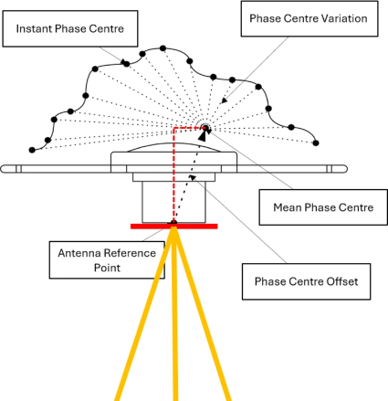
\includegraphics[width=0.35\linewidth]{images/pco_pcv.png}
    \caption{Schéma de principe réalisé pour ce rapport, illustrant le décalage entre le point de référence d'une antenne et son centre de phase.}
    \label{fig:pco_pcv}
\end{figure}

\subsubsection{Décalage du centre de phase (PCO)}

Le \textit{Phase Center Offset} correspond à un vecteur fixe, exprimé dans le
repère propre de l'antenne, reliant le point de référence de l'antenne à son
centre de phase. Ce décalage dépend notamment de la fréquence considérée et du
type d'antenne.

Pour l'antenne du récepteur, le PCO doit être projeté dans la direction
d'arrivée du signal afin de déterminer la contribution correspondante à la
distance mesurée. Pour l'antenne du satellite, le même principe s'applique en
tenant compte de l'orientation de l'antenne dans le repère du satellite.

Le vecteur de visée $\mathbf u_r^s$ est orienté du récepteur vers le satellite.
Après transformation des PCO dans le repère terrestre, le déplacement du
centre de réception raccourcit la distance lorsqu'il est dirigé vers le
satellite, tandis que le déplacement du centre d'émission dans la même
direction l'allonge. Les contributions de premier ordre sont donc

\begin{align}
\Delta_{\mathrm{PCO},r,i}^s
&=-\mathbf u_r^{s\,\mathsf T}\mathbf o_{r,i},
&
\Delta_{\mathrm{PCO},i}^{s}
&=+\mathbf u_r^{s\,\mathsf T}\mathbf o_i^s.
\label{eq:antenna_pco_signs}
\end{align}

avec :

\begin{itemize}
    \item $\mathbf o_{r,i}$ le PCO de l'antenne réceptrice à la fréquence
    $i$, exprimé dans le repère terrestre ;
    \item $\mathbf o_i^s$ le PCO de l'antenne du satellite $s$ à la fréquence
    $i$, exprimé dans le même repère ;
    \item $\Delta_{\mathrm{PCO},r,i}^s$ et
    $\Delta_{\mathrm{PCO},i}^{s}$ leurs contributions signées au modèle de
    distance.
\end{itemize}

\subsubsection{Variation du centre de phase (PCV)}

Le centre de phase réel d'une antenne ne peut cependant pas être décrit par un
simple décalage constant. Sa position apparente varie avec la direction du
signal. Cette variation est appelée \textit{Phase Center Variation} (PCV).

La correction de PCV dépend généralement de l'angle d'élévation et, pour
certaines antennes, de l'azimut du signal. Elle est fournie sous forme de
modèles calibrés pour chaque type d'antenne et pour les différentes fréquences
GNSS.

Les informations nécessaires à la modélisation des PCO et PCV sont
généralement fournies dans les fichiers de calibration d'antennes au format
ANTEX. Ces fichiers permettent notamment d'associer à chaque modèle d'antenne
ses offsets de centre de phase ainsi que ses variations directionnelles pour
les différentes fréquences.

\subsubsection{Application des corrections d'antenne}

On note $\Delta_{\mathrm{PCV},r,i}^s$ et
$\Delta_{\mathrm{PCV},i}^{s}$ les valeurs PCV signées conformément à la
convention ANTEX. Les corrections d'antenne additives utilisées dans les
équations d'observation sont définies par

\begin{align}
\delta_{\mathrm{ant},r,i}^s
&=
\Delta_{\mathrm{PCO},r,i}^s+\Delta_{\mathrm{PCV},r,i}^s,
\\
\delta_{\mathrm{ant},i}^{s}
&=
\Delta_{\mathrm{PCO},i}^{s}+\Delta_{\mathrm{PCV},i}^{s}.
\label{eq:antenna_signed_corrections}
\end{align}

avec :

\begin{itemize}
    \item $\delta_{\mathrm{ant},r,i}^s$ la contribution signée de l'antenne
    réceptrice ;
    \item $\delta_{\mathrm{ant},i}^{s}$ la contribution signée de l'antenne
    satellite ;
    \item le signe positif placé devant ces deux termes dans les modèles PPP
    signifie qu'ils sont ajoutés à la distance entre les points de référence.
\end{itemize}

Cette correction est calculée pour la fréquence et la direction de propagation
considérées. Dans le cas d'une combinaison ionosphère libre, les corrections
associées aux différentes fréquences sont elles-mêmes combinées avec les
mêmes coefficients que les observations correspondantes.

La prise en compte des centres de phase est particulièrement importante pour
un positionnement de précision. En effet, les décalages considérés sont
généralement de l'ordre du centimètre à plusieurs dizaines de centimètres et
peuvent donc devenir significatifs devant la précision recherchée.

\subsection{Effet wind-up}\label{windup}

L'effet wind-up est un effet lié à la polarisation circulaire des signaux GNSS. Lorsque l'antenne d'émission du satellite tourne relativement à l'antenne de réception, la phase de la porteuse reçue varie d'un cycle complet pour chaque rotation de $360^\circ$. Cet effet n'affecte que les mesures de phase et peut s'accumuler sur plusieurs cycles au cours d'une session d'observation prolongée~\cite{wu1993}.

Les vecteurs d'antenne effectifs du satellite et du récepteur, projetés dans le plan perpendiculaire à la ligne de visée, s'écrivent

\begin{align}
\mathbf d^s
&=
\hat{\mathbf x}^s
-(\hat{\mathbf x}^s\cdot\hat{\mathbf k}_r^s)\hat{\mathbf k}_r^s
-\hat{\mathbf k}_r^s\times\hat{\mathbf y}^s,
\\
\mathbf d_r
&=
\hat{\mathbf x}_r
-(\hat{\mathbf x}_r\cdot\hat{\mathbf k}_r^s)\hat{\mathbf k}_r^s
+\hat{\mathbf k}_r^s\times\hat{\mathbf y}_r,
\end{align}

où

\begin{itemize}
    \item $\hat{\mathbf k}_r^s=-\mathbf u_r^s$ est le vecteur unitaire
    orienté du satellite $s$ vers le récepteur $r$, opposé au vecteur de visée ;
    \item $\hat{\mathbf x}^s$, $\hat{\mathbf y}^s$ sont les axes du repère propre de l'antenne du satellite ;
    \item $\hat{\mathbf x}_r$, $\hat{\mathbf y}_r$ sont les axes du repère propre de l'antenne du récepteur.
\end{itemize}

L'angle principal de l'effet wind-up, noté $\Delta\phi^s(t)$, est donné par

\begin{align}
\cos\Delta\phi^s
=
\frac{\mathbf d^s\cdot\mathbf d_r}
{\|\mathbf d^s\|\,\|\mathbf d_r\|},
\end{align}

avec le signe déterminé par

\begin{align}
\operatorname{sign}(\Delta\phi^s)
=
\operatorname{sign}\!\left(
\hat{\mathbf k}_r^s\cdot(\mathbf d^s\times\mathbf d_r)
\right).
\end{align}

L'effet wind-up peut s'accumuler au cours du temps. L'angle principal ne
fournit sa valeur qu'à un nombre entier de tours près. La valeur continue
$\phi_w^s(t)$ est obtenue en choisissant le nombre de tours qui la rend la
plus proche de celle de l'époque précédente :

\begin{align}
\phi_w^s(t)
=
\Delta\phi^s(t)
+2\pi\,\operatorname{round}\!\left(
\frac{\phi_w^s(t-\Delta t)-\Delta\phi^s(t)}{2\pi}
\right),
\end{align}

avec :
\begin{itemize}
    \item $\Delta\phi^s(t)\in[-\pi,\pi]$ l'angle principal calculé à l'époque courante ;
    \item $\phi_w^s(t-\Delta t)$ la valeur continue à l'époque précédente ;
    \item $\operatorname{round}$ l'arrondi à l'entier le plus proche.
\end{itemize}
Ce choix suppose une variation inférieure à un demi-tour entre deux époques.
À l'initialisation, le choix du nombre entier de tours se confond avec
l'ambiguïté de phase. La correction exprimée en mètres est alors

\begin{align}
\delta_{\mathrm{wind\text{-}up},r,i}^s
=
\frac{\lambda_i}{2\pi}\,\phi_w^s(t),
\label{eq:windup}
\end{align}

où $\lambda_i$ est la longueur d'onde de la fréquence $i$ et $\phi_w^s$ est
exprimé en radians. Le facteur $1/(2\pi)$ convertit l'angle en cycles avant la
conversion en mètres. Pour un récepteur statique, l'orientation de l'antenne
de réception est constante~: la variation de l'effet wind-up est
principalement due à l'évolution de l'attitude du satellite et de la géométrie
de visée.


\subsubsection{Retard de Shapiro}\label{shapiro}

La théorie de la relativité générale prédit qu'un signal électromagnétique ne se propage pas dans un espace parfaitement euclidien lorsque celui-ci est soumis au champ gravitationnel d'un corps massif. Le potentiel gravitationnel terrestre induit ainsi un très léger allongement du trajet optique, appelé \textit{retard de Shapiro}~\cite{ashby2003}.

La correction est donnée par

\begin{align}
\delta_{\mathrm{Shapiro},r}^s
=
\frac{2\mu_E}{c^2}
\ln
\left(
\frac{R^s+R_r+\rho_r^s}
     {R^s+R_r-\rho_r^s}
\right),
\end{align}

où

\begin{itemize}
    \item $\mu_E$ est le paramètre gravitationnel terrestre ;
    \item $R^s = \|\mathbf r^s\|$ est la distance entre le centre de la Terre et le satellite ;
    \item $R_r = \|\mathbf r_r\|$ est la distance entre le centre de la Terre et le récepteur ;
    \item $\rho_r^s = \|\mathbf r^s - \mathbf r_r\|$ est la distance géométrique entre le satellite et le récepteur.
\end{itemize}

Cette correction reste faible, de l'ordre de quelques centimètres, mais devient nécessaire dans les applications de positionnement centimétrique telles que le PPP.

\subsubsection{Estimation du retard troposphérique humide}

À l'inverse, la composante humide $ZWD$ est fortement variable dans le temps
et plus difficile à déterminer à partir d'un modèle atmosphérique
déterministe. Dans le traitement PPP, elle est donc introduite comme un paramètre supplémentaire du
problème d'estimation et déterminée conjointement avec les autres inconnues
du positionnement.

Si le vecteur d'état utilisé pour le positionnement est initialement défini
par
\begin{align}
\mathbf x
=
\begin{bmatrix}
\mathbf r_r^{\mathsf T} & c\delta t_r &
B_{r,\mathrm{IF}}^1 & \ldots & B_{r,\mathrm{IF}}^n
\end{bmatrix}^{\mathsf T},
\end{align}
l'estimation de $ZWD$ conduit à l'étendre sous la forme
\begin{align}
\mathbf x
=
\begin{bmatrix}
\mathbf r_r^{\mathsf T} & c\delta t_r & ZWD &
B_{r,\mathrm{IF}}^1 & \ldots & B_{r,\mathrm{IF}}^n
\end{bmatrix}^{\mathsf T}.
\label{eq:state_zwd}
\end{align}

Le paramètre $ZWD$ constitue ainsi une inconnue supplémentaire du système.

\subsubsection{Estimation des gradients troposphériques}

La dépendance azimutale est représentée par deux gradients horizontaux nord et
est selon le modèle de Chen et Herring~\cite{chenHerring1997}.

En réalité, les variations horizontales de pression, de température et
d'humidité peuvent introduire une asymétrie du retard troposphérique autour
du récepteur. Le retard peut alors présenter une dépendance à l'azimut du
satellite, qui n'est pas représentée par le modèle
de l'équation~\eqref{eq:tropo_no_grad}.

Cette asymétrie est ajoutée au modèle de base au moyen de deux paramètres de
gradient horizontal, respectivement orientés selon les directions nord et
est :
\begin{align}
T_r^s(E_r^s,A_r^s)
=
M_{\mathrm{dry}}(E_r^s)ZHD
+
M_{\mathrm{wet}}(E_r^s)ZWD
+
\underbrace{
M_{\mathrm{grad}}(E_r^s)
\left(
G_N\cos A_r^s + G_E\sin A_r^s
\right)
}_{\text{terme de gradient}},
\label{eq:tropo_grad}
\end{align}

avec :

\begin{itemize}
    \item $A_r^s$ l'azimut du satellite ;
    \item $G_N$ et $G_E$ les composantes nord et est du gradient
    troposphérique ;
    \item $M_{\mathrm{grad}}$ la fonction de projection associée ;
\end{itemize}

La formulation détaillée de la fonction de projection utilisée pour les gradients est
présentée en annexe~\ref{annexe:nmf}.

L'introduction de ces deux paramètres nécessite naturellement une extension
du vecteur d'état. Celui-ci devient
\begin{align}
\mathbf x
=
\begin{bmatrix}
\mathbf r_r^{\mathsf T} & c\delta t_r & ZWD & G_N & G_E &
B_{r,\mathrm{IF}}^1 & \ldots & B_{r,\mathrm{IF}}^n
\end{bmatrix}^{\mathsf T}.
\label{eq:state_zwd_grad}
\end{align}


\subsubsection{Observations combinées et paramètres estimés}

L'IF est appliquée au code et à la phase, avec les coefficients de
l'équation~\eqref{new:if}. Après les corrections de biais et d'antenne, et de
wind-up pour la phase, le modèle s'écrit
\begin{align}
P_{r,\mathrm{IF}}^{s,\mathrm{corr}}&=
\mathcal G_{\mathrm{prec},r}^s+\varepsilon_{P,r,\mathrm{IF}}^s,\\
L_{r,\mathrm{IF}}^{s,\mathrm{corr}}&=
\mathcal G_{\mathrm{prec},r}^s+B_{r,\mathrm{IF}}^s+\varepsilon_{L,r,\mathrm{IF}}^s,\\
\mathcal G_{\mathrm{prec},r}^s&=\rho_r^s+c(\delta t_r-\delta t_{\mathrm{prec}}^s)
+T_r^s+\delta_{\mathrm{Sagnac},r}^s+\delta_{\mathrm{Shapiro},r}^s,\\
B_{r,\mathrm{IF}}^s&=\alpha B_{r,1}^s+\beta B_{r,2}^s.
\label{new:ppp_model}
\end{align}
avec :
\begin{itemize}
\item $P_{r,\mathrm{IF}}^{s,\mathrm{corr}}$ et
$L_{r,\mathrm{IF}}^{s,\mathrm{corr}}$ les observations combinées corrigées ;
\item $\mathcal G_{\mathrm{prec},r}^s$ le terme commun, indépendant de la fréquence ;
\item $\delta_{\mathrm{Shapiro},r}^s$ le retard de Shapiro introduit dans
la partie PPP (section~\ref{shapiro}) ;
\item $\delta t_{\mathrm{prec}}^s$ l'horloge satellite issue du produit précis,
avec les corrections requises par sa convention ;
\item $\rho_r^s$ la distance calculée avec l'orbite précise et la position de
station corrigée des marées ;
\item $B_{r,\mathrm{IF}}^s$ l'ambiguïté IF en mètres, qui n'est pas directement
une ambiguïté entière ;
\item les $\varepsilon$ les erreurs résiduelles des observations combinées.
\end{itemize}

Pour une constellation et un modèle troposphérique avec gradients, l'état est
\begin{align}
\mathbf x&=[\,\mathbf r_r^{\mathsf T}\quad c\delta t_r\quad ZWD\quad
G_N\quad G_E\quad B_{r,\mathrm{IF}}^1\quad\cdots\quad
B_{r,\mathrm{IF}}^n\,]^{\mathsf T}.
\label{new:ppp_state}
\end{align}
avec :
\begin{itemize}
\item $\mathbf r_r$ les trois coordonnées de la station ;
\item $n$ le nombre d'arcs d'ambiguïté représentés dans l'état ;
\item les autres paramètres définis précédemment.
\end{itemize}
Les ISB sont ajoutés lorsque plusieurs constellations sont utilisées.

\subsection{Estimation séquentielle et continuité des observations}

Le PPP considéré utilise un filtre de Kalman étendu. À chaque époque, le
filtre prédit l'état et son incertitude à partir de l'époque précédente, puis
les met à jour avec les observations disponibles. Il conserve ainsi
l'information acquise au cours du suivi. Les équations sont données en
annexe~\ref{ann:estimation}.

Chaque paramètre doit recevoir une valeur initiale et une incertitude.
Un modèle d'évolution décrit également les variations admises entre deux
époques. La position d'une station statique, son horloge, la troposphère et
les ambiguïtés n'ont pas les mêmes propriétés temporelles et ne reçoivent
donc pas le même modèle.

La phase de convergence correspond à l'accumulation d'information permettant
de mieux séparer ces paramètres. Le code, bien que moins précis, reste utile
pour initialiser la position, l'horloge et les ambiguïtés.

Une perte de verrouillage est une interruption du suivi de la porteuse.
Elle peut provoquer un saut de cycle, c'est-à-dire une discontinuité du
comptage des cycles. L'ambiguïté antérieure n'est alors plus valable.
Le traitement contrôle les indicateurs du récepteur et des combinaisons
sensibles aux discontinuités. Lorsqu'un saut est détecté ou qu'une interruption
dépasse la durée admise, l'ambiguïté concernée est réinitialisée.
Les mécanismes détaillés sont conservés en annexe~\ref{ann:estimation}.

Le tableau suivant résume les deux traitements retenus dans ce travail.
Ces choix ne constituent pas une définition générale des estimateurs
utilisables en SPP ou en PPP.

\begin{table}[htbp]
\centering
\small
\begin{tabular}{|p{0.20\linewidth}|p{0.32\linewidth}|p{0.34\linewidth}|}
\hline
Élément & SPP retenu & PPP retenu \\\hline
Observations & Code & Code et phase \\\hline
Orbites et horloges & Diffusées & Produits précis \\\hline
Ionosphère & Klobuchar ou IF & IF \\\hline
Troposphère & Modèle a priori & Retard humide estimé, gradients optionnels \\\hline
Estimation & WLS par époque & EKF sur plusieurs époques \\\hline
Ambiguïtés & Absentes & Estimées sur les arcs continus \\\hline
\end{tabular}
\caption{Principales différences entre les traitements SPP et PPP retenus.}
\label{new:summary}
\end{table}

\section{Implémentation avec Orekit}
\label{sec:implementation_nouvelle}
% Partie réservée à la rédaction suivante.
